\documentclass[12pt]{article}
\setlength\parindent{0pt}
\usepackage{fullpage}
%\usepackage[margin=0.5in, paperwidth=13.5in, paperheight=8.4375in]{geometry}
\usepackage[margin=0.5in, paperwidth=8.5in, paperheight=11in]{geometry}

\usepackage{amsmath}
\usepackage{graphicx}
\newcommand{\BI}{\begin{itemize}}
\newcommand{\insp}{\vspace{1in}}
\newcommand{\EI}{\end{itemize}}
\newcommand{\BE}{\begin{enumerate}}
\newcommand{\EE}{\end{enumerate}}
\newcommand{\BS}{\bigskip}
\setlength{\parskip}{4mm}


\pagenumbering{gobble}

\begin{document}
	\begin{center}\sc \Large Tutorial -- The Motion of the Celestial Sphere 
		

\small

	\it 

Up the dome of heaven \\
Like a great hill \\
I watch them marching \\ 
Stately and still \\


\BS

\begin{flushright} \rm --Excerpted from ``Stars'' by Sara Teasdale (1930) \end{flushright}

\end{center}

	\normalsize
	
	{\bf Note and Foreword:} The most difficult part about this material for students is the fact that we too often study from things printed on paper or displayed on screens. These are two-dimensional, but the world is {\it three dimensional}. These exercises are designed to help you think three-dimensionally. But, until we have holographic projectors rather than paper, we have to print it for you.
	
	The {\it absolute best thing you can do} in learning this material is to put your paper down, stand up, and imagine the motion of the stars on the walls and ceiling around you, and use your fingers to point at imaginary stars as they go by. If you do this, the first quiz will likely be quite easy; if you do not, it will likely be very difficult.
	
	Note that your first homework assignment is the last page of this handout.
	

	\section{Directions in the Sky}
	
	The poet above compared the view of the night sky seen from Earth to a ``dome''. Many of us are familiar with the Carrier Dome: half of a sphere, seen from the inside.
	
	We don't have a smooth sphere, but the roof of our auditorium is close enough. Before we can figure out how stars move in our sky, we will need some language to describe where things are located in the sky. 
	
	We have the familiar words {\bf north}, {\bf south}, {\bf east}, and {\bf west} to describe directions on the surface of the Earth. But, since we are describing things in the sky, we will also need the directions {\bf up} and {\bf down}, or {\bf above} and {\bf below}.
	
	Since {\bf up} and {\bf down} are relative, you can relate them to your eye level, or the {\bf horizontal}. So you can say, for instance, things like {\it a little bit above eye level to the east}, or {\it very far up, straight overhead}, or {\it high in the sky to the southwest}.
		
	We've projected four laser-pointer dots around the room. Using this language, describe where they are. (Pretend that they are stars in the sky.)
	
		
	\begin{enumerate}
		\item The green dot on the right-hand wall

\BS\BS\BS
		
		\item The green dot on the ceiling
	
\newpage

		
		\item The red dot on the floor in front of the room
\BS\BS\BS

		
		\item The red dot on the projection screen
\BS\BS\BS
		
	\end{enumerate}

\subsection{The Horizontal and the Horizon}

We can see things below the horizontal (below our eye level) very easily in this room, including some of the laser dots. Astronomers use the word {\it horizon} to describe their ``horizontal'' wherever they are on Earth's surface. 

If we are standing on Earth's surface, can we see stars below ``eye level'', the ``horizontal'', or the ``horizon''? (These words all mean the same thing.) Why or why not?

\insp



\section{The Motion of the Celestial Sphere}

As we saw in the video from the Quad, the stars move as though they are attached to a sphere rotating around Earth, once per day. There is a bright star, the {\it North Star} or {\it Polaris}, near the axis of this sphere that doesn't move much at all. The white line runs from Earth to the North Star.

How would you describe where Polaris is in the sky, using the language of the last section?

\BS\BS\BS\BS

Look now at the computer animation of the stars rotating on the celestial sphere. There are two stars highlighted on the celestial sphere; we will talk about them later. For now, we need to figure out the relationship between the image shown and the cardinal directions. 

The blue sphere in the middle is the Earth, and the white dot on top is the observer. The red grid (shown) is the observer's {\it horizon}. 

As you know, the horizon has four directions: North, South, East, and West.

\begin{enumerate}
	\item Which direction (N/S/E/W) is {\it closest to the camera}? How do you know?
	\insp
	\item Which direction is to the {\it left} of the image? How do you know?
	\insp
	
	\item Which direction is {\it furthest} from the camera? How do you know?
	\insp
	\item Which direction is to the {\it right} of the image? How do you know?
	\insp
\end{enumerate}

\subsection{Following the Purple Star}

Stand up in your seat and trace with your finger the path that the purple star takes in your ``sky''. This is the most important part of the entire exercise! 

Four points are labeled on the orbit. It travels from the white dot to the orange dot to the blue dot to the yellow dot, in order.

\begin{enumerate}
	\item How would you describe the position of the purple star when it is at the {\it white} point on its purple orbit? What star is it below in the sky?
	
	\BS\BS\BS
	
	\item How would you describe its position at the orange point on its purple orbit?
	\BS\BS\BS	
	\item How would you describe its position at the blue point? 
		\BS\BS\BS
	\item How would you describe its position at the yellow point?
		\BS\BS\BS
		
		\item Is this star always visible in the observer's sky?
\end{enumerate}

\subsection{Following the Green Star}

Now, repeat the previous exercise with the green star. This star's motion is close to how the Sun is moving in our sky right now. 

Stand up in your seat and trace with your finger the path that the green star takes in your ``sky''. Again, this is the most important part of this exercise!

Four points are labeled on the orbit. It travels from the white dot to the orange dot to the blue dot to the yellow dot, in order.

\begin{enumerate}
	\item Which direction would you have to look to see the green star when it is at the {\it orange} point on its orbit? What is that star doing in the sky? (Hint: The Sun does this at about the same time every day.)
	
	\BS\BS\BS
	
	\item Which way would you look to see the green star when it is at the {\it blue} point in its orbit?
	\BS\BS\BS	
	\item Which way would you look to see it at the {\it yellow} point? What is it doing now?
	\BS\BS\BS
	\item Which way would you look to see it when it is at the {\it white} point in its orbit?
	\BS\BS\BS
\end{enumerate}

\newpage



\subsection{Drawing the Path of the Purple Star}
	\begin{minipage}{0.5\textwidth}Here is a depiction of our observer's sky looking North, ``into the page''. Suppose that the purple star is located at the white dot at midnight, low on the northern horizon. 
	\end{minipage}
\begin{minipage}{0.5\textwidth}	
	\begin{center}
		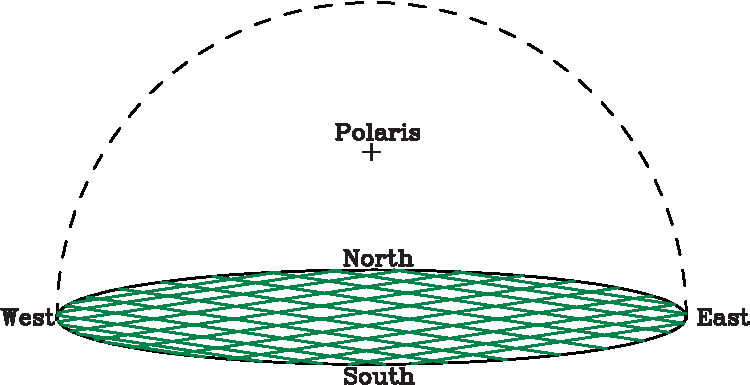
\includegraphics[width=3.5in]{disk-crop.pdf}
	\end{center}
		\end{minipage}
	\begin{enumerate}
	\item Based on what saw found earlier, draw the path that the purple star will take over {\it one day}. Put arrows on that path showing its direction of motion.
		\BS
		
	\item Where will the purple star be at 6 PM? Label it on your diagram, and describe where you would look in the sky to see it.
	\insp
	
	\item This diagram only shows the observer's northern sky. Could we repeat this exercise and draw the path of the {\it purple} star on the animation here? If you can, do it; if you can't, explain why.
	
	\insp \BS\BS
\end{enumerate}

\newpage

(This page left blank.)

\newpage


\begin{center}
	\sc \Large Astronomy 101 Homework 1 \\ \large The Daily Motion of the Sky: Consequences of the Earth's Rotation
\end{center}
\begin{flushright}
\Large

Name: \underline{\hspace{2.7in}}
\BS

Lab Section Number: M0\underline{\hspace{1in}}
\end{flushright}

{\it Instructions: These questions are an extension of the Exercises on the celestial sphere (the first one) and the consequences of the Earth's rotation (the second one). You should tear this page off when you are done so you can turn it in. This is due Thursday, September 9; you will turn them in when you enter the auditorium for class. (We will have a box for you.)}	

\begin{enumerate}
	\item Describe how a star moves after it rises in the East, as seen from Syracuse. Does it move straight up in the sky? Does it travel into the southern or northern sky before setting in the west?
	
	\insp\insp
	
	\begin{minipage}{0.5\textwidth}
	\item Here is a view of the eastern sky, showing the same star that has just risen over the horizon. Which direction will it move after it rises? Draw with an arrow. (You won't be able to draw its whole path, since it sets in the West ``behind you''; that is okay.)
\end{minipage}
\begin{minipage}{0.5\textwidth}
	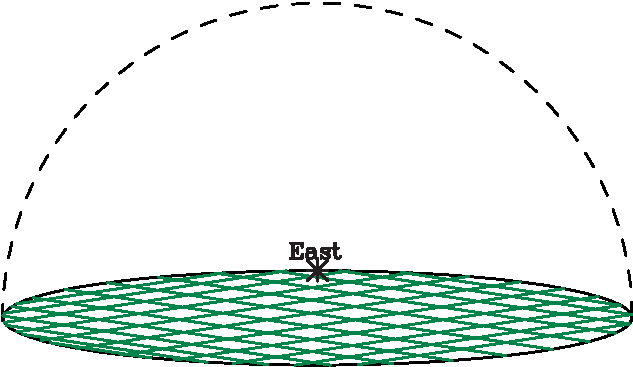
\includegraphics[width=3in]{disk2-crop.pdf}
	\end{minipage}

\BS
\item Are there any stars that we will never get to see in Syracuse? Explain how you know this. If there are stars that we will never get to see, will anyone else get to see them? 

\insp\insp

\item Where would someone at the North Pole see Polaris? What about someone at $5^\circ$ north latitude, just north of the Equator?

\insp\insp

\item We know that we can determine which way is north by finding the North Star in the sky. Could someone in Australia find North in the same way? If not, what could they do instead?

\insp\insp

\item Over the course of {\bf one day}, does the Sun behave similarly to the other stars, or does it do anything different? How do you know?


	
	
\end{enumerate}	

	
\end{document}
	
	
	
	